\documentclass[10pt]{beamer}
\usetheme[
%%% option passed to the outer theme
%    progressstyle=fixedCircCnt,   % fixedCircCnt, movingCircCnt (moving is deault)
  ]{Berlin}
  
% If you want to change the colors of the various elements in the theme, edit and uncomment the following lines

% Change the bar colors:
%\setbeamercolor{Feather}{fg=red!20,bg=red}

% Change the color of the structural elements:
%\setbeamercolor{structure}{fg=red}

% Change the frame title text color:
%\setbeamercolor{frametitle}{fg=blue}

% Change the normal text color background:
%\setbeamercolor{normal text}{fg=black,bg=gray!10}

%-------------------------------------------------------
% INCLUDE PACKAGES
%-------------------------------------------------------

\usepackage[utf8]{inputenc}
\usepackage[english]{babel}
\usepackage[T1]{fontenc}
\usepackage{amsmath}
\usepackage{helvet}
\usepackage{multirow}
\usepackage{graphicx}
\usepackage{comment}
\usepackage[absolute,overlay]{textpos}
\usepackage{tikz}
\usetikzlibrary{arrows,automata,positioning}
\usetikzlibrary{shapes.multipart}
\usetikzlibrary{decorations.markings}

%-------------------------------------------------------
% DEFFINING AND REDEFINING COMMANDS
%-------------------------------------------------------

% colored hyperlinks
%\renewcommand*{\Footnotemark}[1]{\NCC@makefnmark{#1}}
\newcommand{\chref}[2]{
  \href{#1}{{\usebeamercolor[bg]{Feather}#2}}
}
\newcommand{\tuple}[1]{{\langle #1 \rangle}}
\newcommand{\pre}{\mathsf{pre}}     % precondition
\newcommand{\eff}{\mathsf{eff}}     % effect
\newcommand{\cond}{\mathsf{cond}}   % conditional effect

\newcommand{\X}{\mathcal{X}}
\newcommand{\F}{\mathcal{F}}
\newcommand{\A}{\mathcal{A}}
\newcommand{\N}{\mathcal{N}}
\newcommand{\I}{\mathcal{I}}
\newcommand{\real}{\mathbb{R}}
\newcommand{\Dw}{\mathcal{D}}
\newcommand{\Xw}{\mathcal{X}}
\newcommand{\Aw}{\mathcal{A}}
\newcommand{\Rw}{\mathcal{R}}
\newcommand{\OO}{\mathcal{O}}
\newcommand{\tOO}{\wt{\OO}}
\newcommand{\II}[1]{\mathbb{I}{\left\{#1\right\}}}
\newcommand{\PP}[1]{\mathbb{P}\left[#1\right]}
\newcommand{\EE}[1]{\mathbb{E}\left[#1\right]}
\newcommand{\EEs}[2]{\mathbb{E}_{#2}\left[#1\right]}
\newcommand{\PPt}[1]{\mathbb{P}_t\left[#1\right]}
\newcommand{\EEt}[1]{\mathbb{E}_t\left[#1\right]}
\newcommand{\PPi}[1]{\mathbb{P}_i\left[#1\right]}
\newcommand{\EEi}[1]{\mathbb{E}_i\left[#1\right]}
\newcommand{\EEp}[1]{\mathbb{E}_{\pi,P}\left[#1\right]}
\newcommand{\EEcp}[2]{\mathbb{E}_{\pi,P}\left[\left.#1\right|#2\right]}
\newcommand{\PPc}[2]{\mathbb{P}\left[#1\left|#2\right.\right]}
\newcommand{\PPct}[2]{\mathbb{P}_t\left[#1\left|#2\right.\right]}
\newcommand{\PPcc}[2]{\mathbb{P}\left[\left.#1\right|#2\right]}
\newcommand{\PPcct}[2]{\mathbb{P}_t\left[\left.#1\right|#2\right]}
\newcommand{\PPcci}[2]{\mathbb{P}_i\left[\left.#1\right|#2\right]}
\newcommand{\EEc}[2]{\mathbb{E}\left[#1\left|#2\right.\right]}
\newcommand{\EEcc}[2]{\mathbb{E}\left[\left.#1\right|#2\right]}
\newcommand{\EEcs}[3]{\mathbb{E}_{#3}\left[\left.#1\right|#2\right]}
\newcommand{\EEcct}[2]{\mathbb{E}_t\left[\left.#1\right|#2\right]}
\newcommand{\EEcci}[2]{\mathbb{E}_i\left[\left.#1\right|#2\right]}
\renewcommand{\th}{\ensuremath{^{\mathrm{th}}}}
\def\argmin{\mathop{\mbox{ arg\,min}}}
\def\argmax{\mathop{\mbox{ arg\,max}}}
\newcommand{\ra}{\rightarrow}

\newcommand{\norm}[1]{\left\|#1\right\|}
\newcommand{\onenorm}[1]{\norm{#1}_1}
\newcommand{\infnorm}[1]{\norm{#1}_\infty}
\newcommand{\iprod}[2]{\left\langle#1,#2\right\rangle}
\newcommand{\ev}[1]{\left\{#1\right\}}
\newcommand{\pa}[1]{\left(#1\right)}
\newcommand{\bpa}[1]{\bigl(#1\bigr)}
\newcommand{\Bpa}[1]{\Bigl(#1\Bigr)}
\newcommand{\sign}{\mbox{sign}}
\newcommand{\wh}{\widehat}
\newcommand{\wt}{\widetilde}
\newcommand{\transpose}{^\top}

\newcommand{\loss}{\ell}
\newcommand{\hloss}{\wh{\loss}}
\newcommand{\hL}{\wh{L}}
\newcommand{\tZ}{\wt{Z}}
\newcommand{\reg}{\mathfrak{R}}
\newcommand{\hreg}{\widehat{\reg}}
\newcommand{\hr}{\wh{r}}
\newcommand{\hv}{\wh{v}}
\newcommand{\hq}{\wh{q}}
\newcommand{\hmu}{\wh{\mu}}
\newcommand{\hR}{\wh{R}}
\newcommand{\tmu}{\wt{\mu}}
\newcommand{\tN}{\wt{N}}
\newcommand{\RE}[2]{\mbox{RE}\left(\left.#1\right\|#2\right)}
\newcommand{\KL}[2]{\mbox{KL}\left(#1\middle\lVert#2\right)}
\newcommand{\DD}[3]{D_{#3}\left(#1\middle\lVert#2\right)}
\newcommand{\DDC}[2]{\DD{#1}{#2}{C}}
\newcommand{\DDS}[2]{\DD{#1}{#2}{S}}

\newcommand{\trho}{\wt{\rho}}

\definecolor{gold}{rgb}{1,0.75,0}
\definecolor{darkred}{rgb}{0.75,0,0}
\setbeamercolor*{goldc}{fg=black,bg=gold}
\definecolor{darkpurp}{rgb}{0.4,0.2,0.4}
\setbeamercolor*{purpc}{fg=white,bg=darkpurp}
\setbeamercolor*{redc}{fg=white,bg=darkred}
\newcommand{\hG}[1]{\large \textcolor{darkred}{#1}}

\newcommand{\redd}[1]{\textcolor{darkred}{#1}}
\newcommand{\goldd}[1]{\textcolor{gold}{#1}}

\definecolor{ballblue}{rgb}{0.0, 0.53, 0.74}
\definecolor{lightgray}{rgb}{0.85, 0.85, 0.85}

%-------------------------------------------------------
% INFORMATION IN THE TITLE PAGE
%-------------------------------------------------------

\title[] % [] is optional - is placed on the bottom of the sidebar on every slide
{ % is placed on the title page
      \textbf{Machine Learning}
}

\author[Jonsson \& G\'omez]
{      Anders Jonsson \& Vicen\c{c} G\'omez \\
\vspace*{0.5cm}
Master in Intelligence Interactive Systems\\
2021-22\\
\vspace*{0.5cm}
Lecture 1\\
Introduction to Machine Learning
%      {\ttfamily bagchi.bhaskar@cse.iitkgp.ernet.in}
}

\date{}

\AtBeginSection[]
{
   \begin{frame}
       \frametitle{Content}
       \tableofcontents[currentsection]
   \end{frame}
}

%-------------------------------------------------------
% THE BODY OF THE PRESENTATION
%-------------------------------------------------------

\begin{document}

%-------------------------------------------------------
% THE TITLEPAGE
%-------------------------------------------------------

\begin{frame}[plain,noframenumbering] % the plain option removes the header from the title page, noframenumbering removes the numbering of this frame only
  \titlepage % call the title page information from above
\end{frame}

\begin{frame}{Content}{}
\tableofcontents
\end{frame}

\section{General information}

\begin{frame}
  \frametitle{Organization}

  \begin{itemize}
  \item Teachers: Anders Jonsson, Vicen\c{c} G\'omez
  \begin{itemize}
    \item Office: 55.130
    \item Email: \{anders.jonsson,vicen.gomez\}@upf.edu
  \end{itemize}
  \item 10 lectures, 2.5 hours each
  \begin{itemize}
    \item Mostly theory in lectures
	\item Several lab sessions (lectures 3, 5, 7 and 8)
  \end{itemize}
  \item Homeworks and programming exercises
  \item Final exam in December
  \end{itemize}
\end{frame}

\begin{frame}
  \frametitle{Evaluation}

  \begin{itemize}
  \item Final grade is calculated as follows:
  \begin{enumerate}
	\item Homeworks: $4\times 5\%=20\%$
    \item Programming exercises: $4\times 10\%=40\%$
    \item Final exam: $40\%$
  \end{enumerate}
  \item To pass the course, need a passing grade in all parts
  \end{itemize}
\end{frame}

\begin{frame}
  \frametitle{Objective}

  \begin{itemize}
  \item {\color{red} Understand the mathematical principles of machine learning}
  \item Solve mathematical exercises related to machine learning theory
  \item Recognize different types of machine learning problem
  \item Choose and implement appropriate machine learning algorithms
  \item Evaluate learning outcome and compare different algorithms
  \item Select appropriate values of hyperparameters through validation
  \end{itemize}
\end{frame}

\begin{frame}
  \frametitle{Prerequisites}

  Students are expected to have basic knowledge in these topics:
  \begin{itemize}
  \item Linear algebra
  \item Calculus
  \item Probability theory/statistics
  \end{itemize}
\end{frame}

\begin{frame}
  \frametitle{Topics}

  \begin{itemize}
    \item[1.] Introduction to machine learning (Anders)
	% Problem 1.4
    \item[2.] Linear models (Anders)
    % Problems 2.1-2.4
    \item[3.] Bias-variance tradeoff and overfitting (Anders) {\color{red} + LS \#1}
    % Problems 1.10, 2.22
	\item[4.] Optimization and gradient descent (Anders)
    % Problem 4.24
	\item[5.] Common algorithms for supervised learning (Anders) {\color{red} + LS \#2}
  	\item[6.] Unsupervised learning (Anders)
    \item[7.] Deep Learning and Applications I (Anders) {\color{red} + LS \#3}
    \item[8.] Deep Learning and Applications II (Vicen\c{c}) {\color{red} + LS \#4}
    \item[9.] Bayesian learning and inference (Vicen\c{c})
    \item[10.] Introduction to probabilistic graphical models (Vicen\c{c})
    % Implement a model-free RL algorithm for Blackjack
  \end{itemize}
\end{frame}

\newcommand\Wider[2][5em]{%
\makebox[\linewidth][c]{%
  \begin{minipage}{\dimexpr\textwidth+#1\relax}
  \raggedright#2
  \end{minipage}%
  }%
}

{\setbeamercolor{background canvas}{bg=lightgray}
\begin{frame}
  \frametitle{Books}
\Wider{
  \begin{tabular}{lll}
  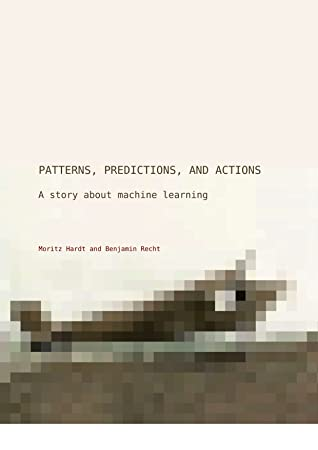
\includegraphics[height=5cm]{images/patterns.jpg} & 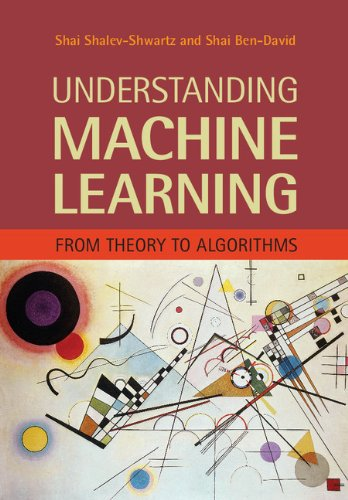
\includegraphics[height=5cm]{images/UML.jpg} & 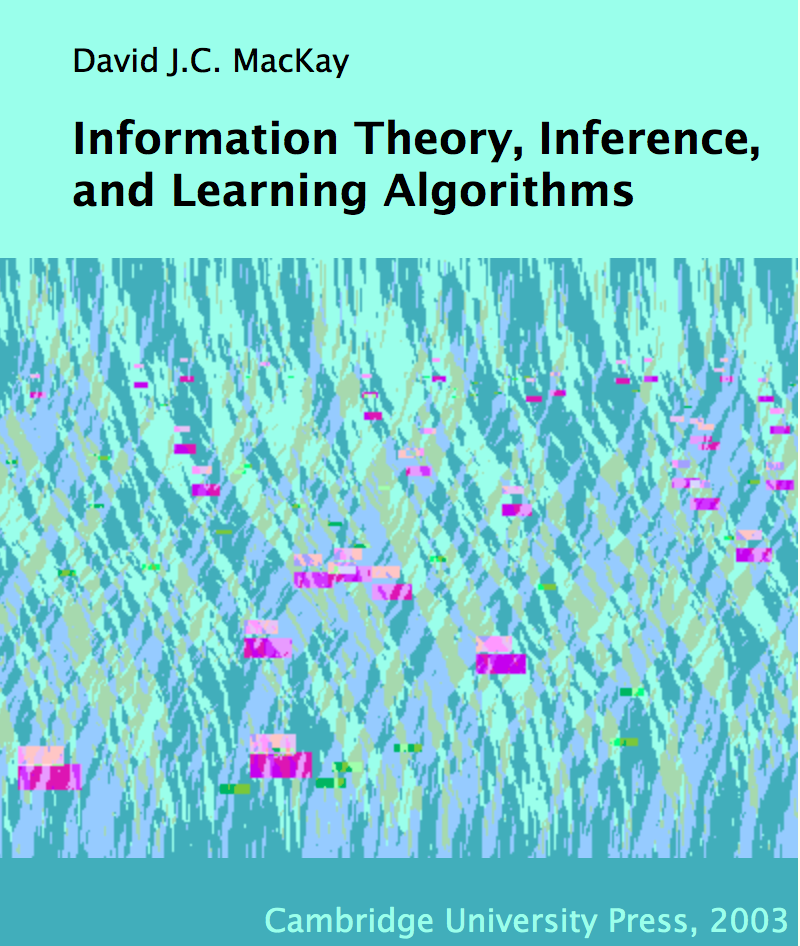
\includegraphics[height=5cm]{images/it.png}
  \end{tabular}
}
\end{frame}}

\section{Introduction to Machine Learning}

\begin{frame}
  \frametitle{Definition of machine learning}

  From Wikipedia:
  ``Machine learning (ML) is the study of {\color{red} computer algorithms} that can {\color{blue} improve automatically} through experience and by the use of data. Machine learning algorithms build a {\color{cyan} model} based on {\color{green} sample data} [...] in order to make {\color{orange} predictions or decisions}.''
\end{frame}

\begin{frame}
  \frametitle{Machine learning problems}

  In which of the following problems can machine learning help?
  \begin{itemize}
	\item Predict on which weekday the next market crash will occur
	\item Classify an email as spam or not spam
	\item Find the shortest path between two nodes in a graph
	\item Recognize cancerous cells in the X-ray image of a patient
	\item Guess when the next world-wide pandemia will occur
  \end{itemize}
\end{frame}

\begin{frame}
  \frametitle{Characteristics of machine learning problems}

  \begin{itemize}
	\item There exists an underlying {\color{red} pattern} that we can exploit
	\item Describing (or programming) the pattern is difficult
	\item However, one can obtain many {\color{green} observations} ({\color{green} data}) of the pattern
	\item Machine learning algorithms can {\color{blue} learn} the pattern (or an approximation) from data
  \end{itemize}
\end{frame}

\begin{frame}
  \frametitle{Machine learning problems}

  In which of the following problems can machine learning help?
  \begin{itemize}
	\item Predict on which weekday the next market crash will occur
	\item {\color{green} Classify an email as spam or not spam}
	\item Find the shortest path between two nodes in a graph
	\item {\color{green} Recognize cancerous cells in the X-ray image of a patient}
	\item Guess when the next world-wide pandemia will occur
  \end{itemize}
\end{frame}

\begin{frame}
  \frametitle{Intuition}
  \centering{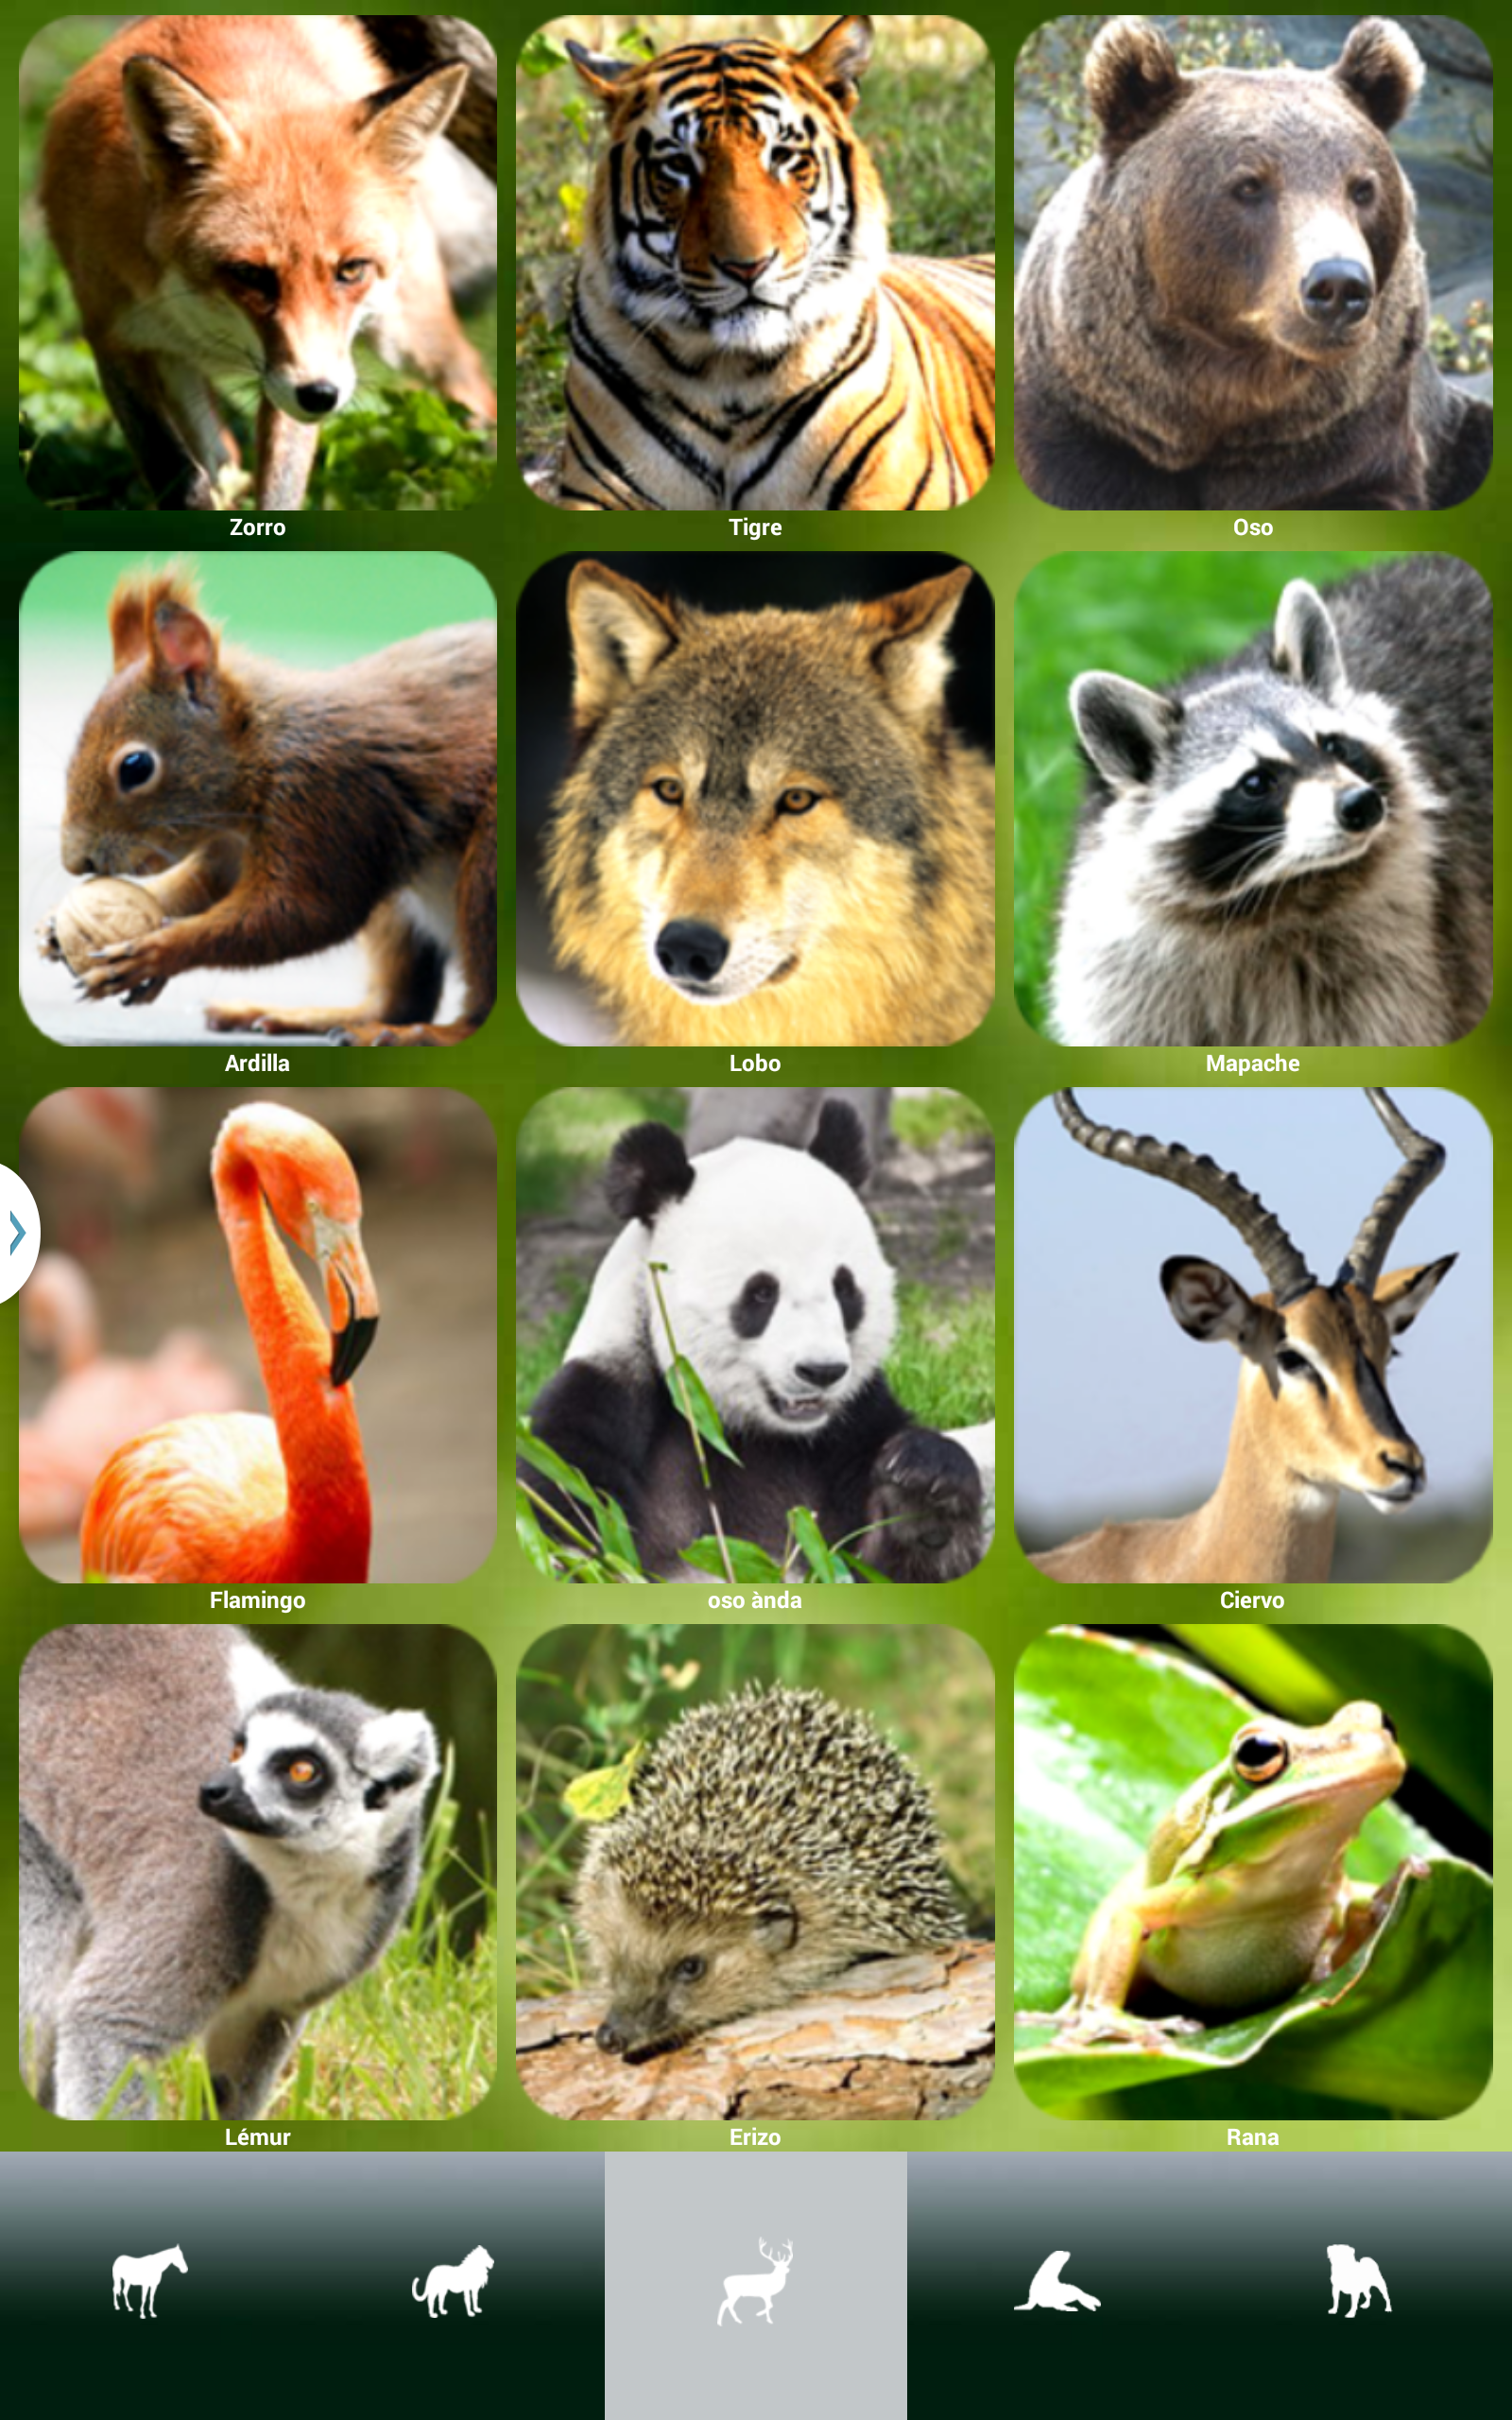
\includegraphics[height=4cm]{images/animals.png}}
  \begin{itemize}
	\item There exists a set of objects or concepts that we want to analyze
	\item {\color{red} Key assumption}: objects with similar features behave similarly
	\item If this assumption does not hold, learning is hopeless
  \end{itemize}
\end{frame}

\begin{frame}
  \frametitle{Example [Understanding Machine Learning]}
  \begin{center}
  \begin{tabular}{ll}
  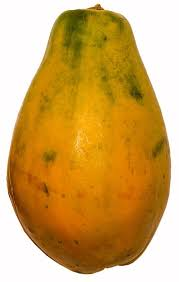
\includegraphics[height=3cm]{images/papaya.jpeg} & 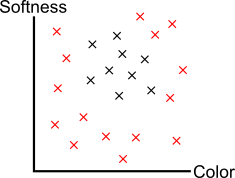
\includegraphics[height=3cm]{images/papaya1.png}
  \end{tabular}
  \end{center}
  \begin{itemize}
	\item Papayas can be described by two features: softness and color
	\item Papayas are either tasty ({\textsf x}) or not tasty ({\color{red} \textsf x})
	\item We can obtain many {\color{blue} observations} of papayas: softness, color, and tastiness
  \end{itemize}
\end{frame}

\begin{frame}
  \frametitle{Example (cont.)}
  \begin{center}
  \begin{tabular}{ll}
  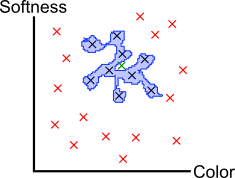
\includegraphics[height=3cm]{images/papaya2.png} & 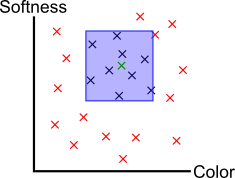
\includegraphics[height=3cm]{images/papaya3.png}
  \end{tabular}
  \end{center}
  \begin{itemize}
	\item Machine learning algorithms attempt to find a {\color{blue} pattern} that explains the relationship between {\color{green} features} (softness, color) and {\color{orange} label} (tastiness)
	\item Many possible patterns exist for explaining this relationship!
  \end{itemize}
\end{frame}

\begin{frame}
  \frametitle{Prediction}
  \vspace*{0.5cm}
  \begin{center}
  \begin{tikzpicture}[overlay]
	\node at (-2,0) {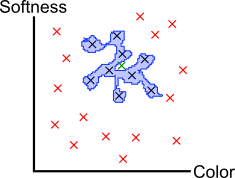
\includegraphics[height=3cm]{images/papaya2.png}};
	\draw[color=orange,thick=2pt] (-2.3,-0.2) -- (-2.18,-0.05);
	\draw[color=orange,thick=2pt] (-2.3,-0.05) -- (-2.18,-0.2);
	\node at (2,0) {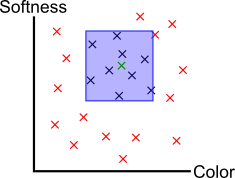
\includegraphics[height=3cm]{images/papaya3.png}};
	\draw[color=orange,thick=2pt] (1.7,-0.2) -- (1.82,-0.05);
	\draw[color=orange,thick=2pt] (1.7,-0.05) -- (1.82,-0.2);
  \end{tikzpicture}
  \end{center}
  \vspace*{1.5cm}
  \begin{itemize}
	\item Given an unseen papaya ({\color{orange} \textsf x}), {\color{blue} predict} whether or not it is tasty
	\item Record features (softness, color) and use pattern model to predict tastiness 
	\item Prediction depends on model! Need a way to measure {\color{purple} performance} of models
  \end{itemize}
\end{frame}

\begin{frame}
  \frametitle{Areas of machine learning}
  \begin{itemize}
	\item {\color{red} Supervised learning}: data contains (feature,label) pairs, objective is to predict target for unseen examples
	\item {\color{red} Unsupervised learning}: data only contains feature examples, objective is to find patterns in features
	\item {\color{red} Reinforcement learning}: algorithms can perform {\color{blue} actions} that modify features, objective is to perform actions that maximize long-term {\color{green} reward}
  \end{itemize}
\end{frame}

\section{Mathematical formulation of supervised learning}

\begin{frame}
  \frametitle{Domain set}
  \begin{itemize}
	\item Assume that there exists a set of {\color{red} features} $\mathcal{X}^1,\ldots,\mathcal{X}^d$
	\item Objects or concepts are described by {\color{green} feature vectors} $(x^1,\ldots,x^d)$
	\item An {\color{cyan} input} is given by $x = (x^1,\ldots,x^d) \in \mathcal{X}^1\times\cdots\times\mathcal{X}^d \equiv \mathcal{X}$
	\item $\mathcal{X}$ is called the {\color{blue} domain set}, {\color{blue} input set}, or {\color{blue} sample space}
	\item $d$ is the number of {\color{purple} dimensions}, e.g. $d=2$ in the papaya example
  \end{itemize}
\end{frame}

\begin{frame}
  \frametitle{Input distribution}
  \begin{center}
	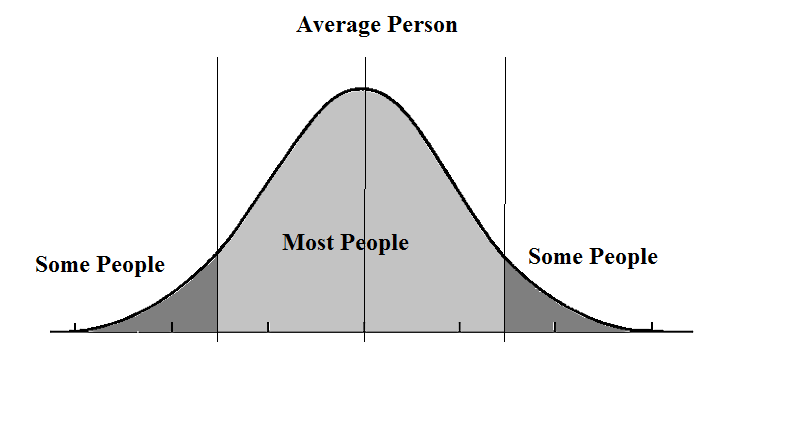
\includegraphics[height=3.5cm]{images/bell.png}
  \end{center}
  \begin{itemize}
	\item Not all inputs are equally likely
	\item Assume that inputs follow a {\color{red} probability distribution} $\mathcal{D}$
	\item We can {\color{green} sample} an input $x\sim\mathcal{D}$ from the probability distribution
  \end{itemize}
\end{frame}

\begin{frame}
  \frametitle{Target set}
  \begin{itemize}
	\item Target set (label space) $\mathcal{Y}$ represents what we want to {\color{blue} predict}
	\item The machine learning problem depends on the form of $\mathcal{Y}$:\\

	\vspace*{0.3cm}

	\begin{tabular}{ll}
		$\mathcal{Y}=\{c_1,\ldots,c_k\}$: & {\color{red} classification} (target is a class)\\
		$\mathcal{Y}=\mathbb{R}$: & {\color{red} regression} (target is a real number)\\
		$\mathcal{Y}=[0,1]$: & {\color{red} logistic regression} (target is a probability)
	\end{tabular}
	\vspace*{0.3cm}
	\item For example, $\mathcal{Y}=\{\mathrm{tasty},\mathrm{not\;tasty}\}$ in the papaya example
  \end{itemize}
\end{frame}

\begin{frame}
  \frametitle{Labelling function}
  \begin{itemize}
	\item The unknown {\color{red} pattern} that we are trying to learn
	\item Mathematically, the pattern is a {\color{blue} labelling function} $f:\mathcal{X} \rightarrow \mathcal{Y}$
	\item For a given input $x\in\mathcal{X}$, the label is $y=f(x)\in\mathcal{Y}$
	\item In practice, labelling is noisy, and two identical inputs may have different labels
  \end{itemize}
\end{frame}

\begin{frame}
  \frametitle{Training set}
  \begin{itemize}
	\item Data is obtained by observing multiple labelled examples
	\item The result is a {\color{red} training set} $S=((x_1,y_1),\ldots,(x_m,y_m))$
	\item Each data point $(x_i,y_i)$, $1\leq i\leq m$, consists of an input $x_i\sim\mathcal{D}$ and a label $y_i=f(x_i)$
	\item Technically, $S$ is a {\color{green} sequence} and not a set, since two distinct data points $(x_i,y_i)$ and $(x_j,y_j)$, $1\leq i<j\leq N$, may be identical
	\item Some algorithms process the data points in $S$ sequentially
  \end{itemize}
\end{frame}

\begin{frame}
  \frametitle{Supervised learning problem}
  To summarize, a supervised learning problem consists of:
  \begin{itemize}
	\item A domain set $\mathcal{X}=\mathcal{X}^1\times\cdots\times\mathcal{X}^d$
	\item An {\color{red} unknown} probability distribution $\mathcal{D}$ on $\mathcal{X}$
	\item A target set $\mathcal{Y}$
	\item An {\color{red} unknown} labelling function $f:\mathcal{X}\rightarrow\mathcal{Y}$
	\item A training set $S=((x_1,y_1),\ldots,(x_m,y_m))$ {\color{blue} sampled} from $\mathcal{D}$ and $f$
  \end{itemize}
\end{frame}

\begin{frame}
  \frametitle{Hypothesis class}
  \begin{center}
	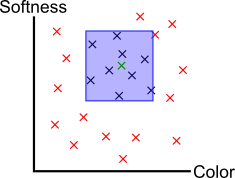
\includegraphics[height=3cm]{images/papaya3.png}
  \end{center}
  \begin{itemize}
	\item Since the space of functions is enormous, the learner usually {\color{red} restricts} the space of candidate functions
	\item Hypothesis class $\mathcal{H}$: set of functions considered by the learner
	\item Each hypothesis $h\in\mathcal{H}$ is a function from $\mathcal{X}$ to $\mathcal{Y}$, i.e.~$h:\mathcal{X}\rightarrow\mathcal{Y}$
	\item Papaya example: set of rectangles in two dimensions
  \end{itemize}
\end{frame}

\begin{frame}
  \frametitle{Loss function}
  \begin{itemize}
	\item Need a way to measure the {\color{green} performance} of a hypothesis $h\in\mathcal{H}$
	\item {\color{blue} Loss function} $\ell:\mathcal{Y}\times\mathcal{Y}\rightarrow \mathbb{R}$: measures the {\color{red} error} between a prediction $\hat{y}$ and the true label $y$
	\item Loss is a (non-negative) {\color{orange} cost}: lower is better
	\item Many different loss functions exist
	\begin{itemize}
	\item Classification or 0-1 loss: $\ell(\hat{y},y)=[\hat{y} \neq y]$
	\item Squared loss: $\ell(\hat{y},y) = (\hat{y} - y)^2$
	\end{itemize}
  \end{itemize}
\end{frame}

\begin{frame}
  \frametitle{True loss vs. training loss}
  \begin{itemize}
	\item Loss can measure the {\color{green} performance} of a hypothesis $h\in\mathcal{H}$
	\item {\color{orange} True loss} $L_{\mathcal{D},f}(h)$, also known as {\color{orange} generalization error} or {\color{orange} risk}, measures the mistakes of $h$ on the entire {\color{blue} domain set $\mathcal{X}$}
	\[
	L_{\mathcal{D},f}(h) = \mathbb{E}_{x\sim\mathcal{D}} \left\{ \ell(h(x),f(x)) \right\}
	\]
	\item {\color{red} Training loss} $L_S(h)$, also known as {\color{red} empirical risk}, measures the mistakes of $h$ on the {\color{cyan} training set $S=((x_1,y_1),\ldots,(x_m,y_m))$}
	\[
	L_S(h) = \frac 1 m \sum_{i=1}^m \ell(h(x_i),y_i)
	\]
  \end{itemize}
\end{frame}

\begin{frame}
  \frametitle{Learning algorithm}
  \begin{center}
	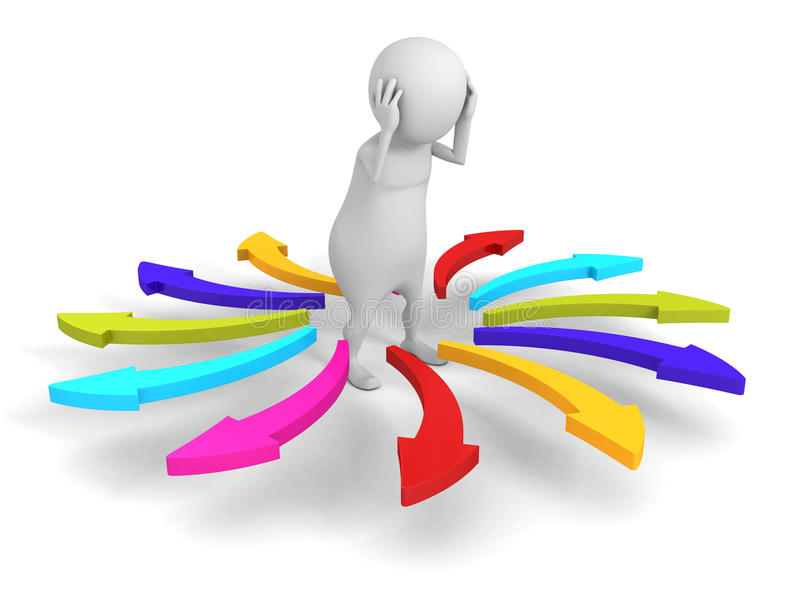
\includegraphics[height=3cm]{images/choices.jpg}
  \end{center}
  \begin{itemize}
	\item A learning algorithm should output a hypothesis $h\in\mathcal{H}$ that approximates $f$ well
	\item We would like $h$ to minimize the true loss $L_{\mathcal{D},f}(h)$
	\item However, $L_{\mathcal{D},f}(h)$ is {\color{red} unobservable} since $\mathcal{D}$ and $f$ are unknown
  \end{itemize}
\end{frame}

\begin{frame}
  \frametitle{Empirical risk minimization}
  \begin{itemize}
	\item Basic principle of supervised learning
	\item Given a hypothesis class $\mathcal{H}$ and a training set $S$, return the hypothesis that {\color{red} minimizes the empirical risk} (i.e.~training loss)
	\item Formally,
	\[
	h_S=\mathrm{ERM}_\mathcal{H}(S) \in \arg\min_{h\in\mathcal{H}}L_S(h),
	\]
	\item Note that if $f\in\mathcal{H}$, $L_S(h_S)=0$
  \end{itemize}
\end{frame}

\begin{frame}
  \frametitle{Supervised learning}
  To summarize, given a supervised learning problem, the learner chooses the following:
  \begin{itemize}
	\item A hypothesis class $\mathcal{H}$ of candidate labelling functions
	\item A loss function $\ell:\mathcal{Y}\times\mathcal{Y}\rightarrow \mathbb{R}$
	\item An algorithm $\mathcal{A}$ that minimizes the empirical risk
  \end{itemize}
\end{frame}

\begin{frame}
  \frametitle{Generalization properties}
  \begin{itemize}
	\item Trivially, we have
	\[L_{\mathcal{D},f}(h) = L_S(h) + {\color{red} (L_{\mathcal{D},f}(h) - L_S(h))}\]
	\item For a fixed $h\in\mathcal{H}$, how well does $L_S(h)$ approximate $L_{\mathcal{D},f}(h)$?
	\item Depends on quality of the {\color{blue} training set $S=((x_1,y_1),\ldots,(x_m,y_m))$}
	\item If we are {\color{red} unlucky}, $L_S(h)$ is not representative of $L_{\mathcal{D},f}(h)$
	\item With {\color{green} high probability}, $L_S(h)$ approximates $L_{\mathcal{D},f}(h)$ well
  \end{itemize}
\end{frame}

\begin{frame}
  \frametitle{Bin analogy}
  \begin{center}
	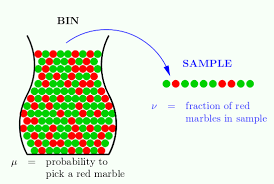
\includegraphics[height=4cm]{images/bins.png}
  \end{center}
  \begin{itemize}
	\item Large bin with red and green marbles, proportion red/green = $\mu$
	\item Randomly pick $m$ marbles, record proportion $\nu$ of red marbles
	\item Hoeffding's inequality (holds for any $\epsilon$):
	\[
	\mathbb{P}\left[|\nu - \mu| > \epsilon\right] \leq 2 e^{-2m\epsilon^2}
	\]
  \end{itemize}
\end{frame}

\begin{frame}
  \frametitle{Bin analogy}
  \begin{center}
	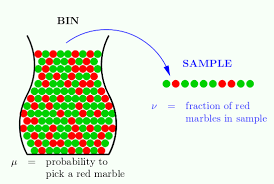
\includegraphics[height=4cm]{images/bins.png}
  \end{center}
  \begin{itemize}
	\item Marbles: inputs in $\mathcal{X}$, {\color{red} red}: $h(x)\neq f(x)$, {\color{green} green}: $h(x)=f(x)$ 
	\item Then $L_{\mathcal{D},f}(h)=\mu$, $L_S(h)=\nu$
	\item Hoeffding's inequality:
	\[
	\mathbb{P}\left[|L_S(h) - L_{\mathcal{D},f}(h)| > \epsilon\right] \leq 2 e^{-2m\epsilon^2}
	\]
  \end{itemize}
\end{frame}

\begin{frame}
  \frametitle{Growth of upper bound}
  \begin{center}
  \begin{tikzpicture}
  \draw[thick,->] (0,0) -- (5,0) node[right]{$m$};
  \draw[thick,->] (0,0) -- (0,3) node[above]{$2 e^{-2m\epsilon^2}$};
  \draw[red,domain=0:5] plot (\x,{2.5*pow(2,-\x)});
  \end{tikzpicture}
  \end{center}
  \begin{itemize}
	\item Probability of $S$ being {\color{red} bad} decreases as a function of $m$
  \end{itemize}
\end{frame}

\begin{frame}
  \frametitle{Generalization}
  \begin{itemize}
	\item Empirical risk minimization returns a hypothesis
	\[
	h_S=\mathrm{ERM}_\mathcal{H}(S) \in \arg\min_{h\in\mathcal{H}}L_S(h)
	\]
	\item How well does $L_S(h_S)$ approximate $L_{\mathcal{D},f}(h_S)$?
	\item {\color{red} Bias} due to the fact that we select $h$ with {\color{blue} smallest $L_S(h)$}
  \end{itemize}
\end{frame}

\begin{frame}
  \frametitle{Coin flipping}
  \begin{tabular}{ccccc}
	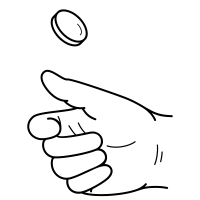
\includegraphics[height=2cm]{images/coinflip.png} &
	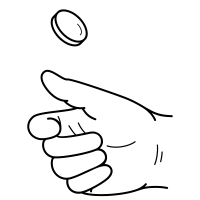
\includegraphics[height=2cm]{images/coinflip.png} &
	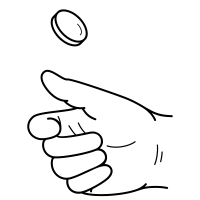
\includegraphics[height=2cm]{images/coinflip.png} &
	$\cdots$ &
	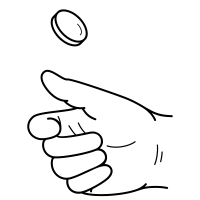
\includegraphics[height=2cm]{images/coinflip.png}
  \end{tabular}

  \vspace*{.5cm}

  \begin{itemize}
	\item Assume that K people each flip a coin 10 times
	\item In expectation, each person will get 5 heads and 5 tails
	\item However, probability of getting 10 heads (or 10 tails) $\approx 0.1\%$
	\item Analogously, the $h$ with smallest $L_S(h)$ may have been {\color{green} lucky}
  \end{itemize}
\end{frame}

\begin{frame}
  \frametitle{Generalization}
  \begin{itemize}
	\item For {\color{red} each} hypothesis $h\in\mathcal{H}$, bound the probability of $S$ being {\color{red} bad}
	\[
	2 e^{-2m\epsilon^2} + 2 e^{-2m\epsilon^2} + \ldots + 2 e^{-2m\epsilon^2}
	\]
	\item {\color{green} Union bound} on Hoeffding's inequality yields
	\[
	\mathbb{P}\left[|L_S(h_S) - L_{\mathcal{D},f}(h_S)| > \epsilon\right] \leq 2 {\color{red} |\mathcal{H}|}e^{-2m\epsilon^2}
	\]
  \end{itemize}
\end{frame}

\begin{frame}
  \frametitle{Noisy labels}
  \begin{itemize}
	\item In practice, two identical inputs may have different labels
	\item As an alternative to the labelling function $f$, we can model this as a {\color{red} conditional probability distribution $\mathbb{P}(y|x)$}
	\item On input $x$, the label is $y$ with probability $\mathbb{P}(y|x)$
	\item Even more compactly, we can define a {\color{blue} joint probability distribution $\mathcal{D}$} on $\mathcal{X}\times\mathcal{Y}$ and sample data points $(x,y)\sim\mathcal{D}$
  \end{itemize}
\end{frame}

\section{Basic algorithms}

\begin{frame}
  \frametitle{Na\"ive empirical risk minimization}
  \begin{block}{Empirical risk minimization}
	\begin{itemize}
	\item For each hypothesis $h\in\mathcal{H}$, compute the loss $L_S(h)$
	\item Return hypothesis with smallest $L_S(h)$
	\end{itemize}
  \end{block}
  Iterates over {\color{red} all hypotheses} in $\mathcal{H}$ and {\color{red} all data points} in $S$!
\end{frame}

\begin{frame}
  \frametitle{Online learning}
  \begin{center}
	
\includegraphics[height=3cm]{images/stream.png}
  \end{center}
  \begin{itemize}
	\item Process data points one at a time
	\item Update the candidate hypothesis after seeing each data point
	\item {\color{blue} Sequential}: order of the data points matter!
	\item For the moment, {\color{green} assume $|\mathcal{Y}|=2$, $f\in\mathcal{H}$ and finite $|\mathcal{H}|$}
  \end{itemize}
\end{frame}

\begin{frame}
  \frametitle{Consistent learner}
  \begin{block}{Consistent learner}
	\begin{itemize}
	\item Initialize $\mathcal{H}_1 \gets \mathcal{H}$
	\item For $t=1,2,\ldots$
	\begin{enumerate}
	\item Get $x_t$
	\item Pick some $h\in\mathcal{H}_t$ and predict $h(x_t)$
	\item Get $y_t=f(x_t)$ and update $\mathcal{H}_{t+1}=\{h\in\mathcal{H}_t:h(x_t)=y_t\}$
	\end{enumerate}
	\end{itemize}
  \end{block}
\end{frame}

\begin{frame}
  \frametitle{Consistent learner}
  \begin{theorem}
	The consistent learner will make at most $|\mathcal{H}|-1$ mistakes.
  \end{theorem}
\end{frame}

\begin{frame}
  \frametitle{Halving learner}
  \begin{block}{Halving learner}
	\begin{itemize}
	\item Initialize $\mathcal{H}_1 \gets \mathcal{H}$
	\item For $t=1,2,\ldots$
	\begin{enumerate}
	\item Get $x_t$
	\item Pick \textsc{Majority}$(h(x_t):h\in\mathcal{H}_t)$
	\item Get $y_t=f(x_t)$ and update $\mathcal{H}_{t+1}=\{h\in\mathcal{H}_t:h(x_t)=y_t\}$
	\end{enumerate}
	\end{itemize}
  \end{block}
\end{frame}

\begin{frame}
  \frametitle{Halving learner}
  \begin{theorem}
	The halving learner will make at most $\log_2(|\mathcal{H}|)$ mistakes.
  \end{theorem}
\end{frame}

\begin{frame}
  \frametitle{Halving learner}
  Advantages:
  \begin{itemize}
	\item Makes very few mistakes!
	\item No need to store a training set or compute a loss function
  \end{itemize}
  Disadvantages:
  \begin{itemize}
	\item Assumes $f\in\mathcal{H}$ (else we may exclude best hypothesis)
	\item In each time step, iterates over all hypotheses in $\mathcal{H}$!
  \end{itemize}
\end{frame}

\begin{frame}
  \frametitle{Algorithmic properties}

  \begin{center}
  \begin{tikzpicture}[overlay]
	\node at (0,0) {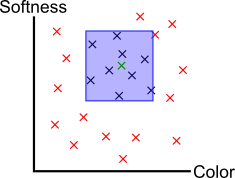
\includegraphics[height=3cm]{images/papaya3.png}};
	\draw (0.02,0.32) circle (.75cm);
  \end{tikzpicture}
  \end{center}

  \vspace*{1cm}

  \begin{itemize}
	\item We cannot always assume $f\in\mathcal{H}$ and $|\mathcal{H}|$ small (or even finite)
	\item Important that algorithms are computationally {\color{green} efficient}
	\item Even minimizing the empirical risk is often expensive (NP-hard)
	\item Usually algorithms are {\color{red} specialized} to the hypothesis class $\mathcal{H}$ and loss function $\ell$
  \end{itemize}
\end{frame}

\begin{frame}
  \frametitle{$k$ nearest neighbors}
  \begin{center}
	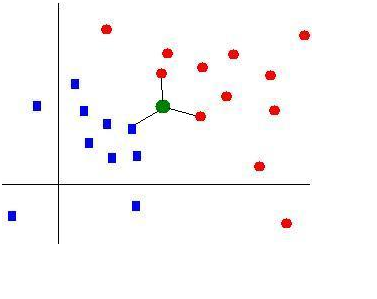
\includegraphics[height=3cm]{images/knn.png}
  \end{center}
  \begin{itemize}
  \item Assume that there exists a {\color{blue} distance function} $\rho:\mathcal{X}\times\mathcal{X}\rightarrow\mathbb{R}$
  \item Given $S=((x_1,y_1),\ldots,(x_m,y_m))$ and $x\in\mathcal{X}$, let $\pi_1(x),\ldots,\pi_m(x)$ be a {\color{red} permutation} of $1,\ldots,m$ according to their distance from $x$
  \item $k$ nearest neighbors: make prediction based on the $k$ nearest neighbors in $S$
  \end{itemize}
\end{frame}

\begin{frame}
  \frametitle{$k$ nearest neighbors}
  \begin{block}{$k$ nearest neighbors}
	\begin{itemize}
	\item Get input $x$
	\item Return \textsc{Majority}$(y_{\pi_i(x)}:i\leq k)$
	\end{itemize}
  \end{block}
  No need for a hypothesis class or a loss function!
\end{frame}

\begin{frame}
  \frametitle{$k$ nearest neighbors}
  \begin{theorem}
	$\mathbb{E}_{S\sim\mathcal{D},f} [L_{\mathcal{D},f}(h_S)] \leq 2 L_{\mathcal{D},f}(h^*) + 4c\sqrt{d}m^{-\frac 1 {d+1}}$
  \end{theorem}
  $h^*$ is the {\color{orange} optimal} hypothesis\\
  Constant $c$ bounds how much $f$ can {\color{blue} change} as a function of distance
\end{frame}

\section{Exercises}

\begin{frame}
  \frametitle{Consistent learner}
  Prove that the consistent learner makes at most $|\mathcal{H}|-1$ mistakes
  \begin{block}{Consistent learner}
	\begin{itemize}
	\item Initialize $\mathcal{H}_1 \gets \mathcal{H}$
	\item For $t=1,2,\ldots$
	\begin{enumerate}
	\item Get $x_t$
	\item Pick some $h\in\mathcal{H}_t$ and predict $h(x_t)$
	\item Get $y_t=f(x_t)$ and update $\mathcal{H}_{t+1}=\{h\in\mathcal{H}_t:h(x_t)=y_t\}$
	\end{enumerate}
	\end{itemize}
  \end{block}
\end{frame}

\begin{frame}
  \frametitle{Consistent learner}
  \begin{itemize}
	\item Assume the algorithm makes a mistake in round $t$
	\pause
	\item Then the hypothesis $h$ used for prediction will {\color{red} not} be part of $\mathcal{H}_{t+1}$
	\pause
	\item It follows that $|\mathcal{H}_{t+1}|\leq|\mathcal{H}_t|-1$
	\pause
	\item After $k$ mistakes, $|\mathcal{H}_t| \leq |\mathcal{H}| - k$
	\pause
	\item Since $f\in\mathcal{H}$ and $f$ never makes mistakes, $|\mathcal{H}_t|\geq 1$ for each $t$
	\pause
	\item Hence $|\mathcal{H}| - k \geq |\mathcal{H}_t| \geq 1$, which is equivalent to $k \leq |\mathcal{H}| - 1$
  \end{itemize}
\end{frame}

\begin{frame}
  \frametitle{Halving learner}
  Prove that the halving learner makes at most $\log_2(|\mathcal{H}|)$ mistakes
  \begin{block}{Halving learner}
	\begin{itemize}
	\item Initialize $\mathcal{H}_1 \gets \mathcal{H}$
	\item For $t=1,2,\ldots$
	\begin{enumerate}
	\item Get $x_t$
	\item Pick \textsc{Majority}$(h(x_t):h\in\mathcal{H}_t)$
	\item Get $y_t=f(x_t)$ and update $\mathcal{H}_{t+1}=\{h\in\mathcal{H}_t:h(x_t)=y_t\}$
	\end{enumerate}
	\end{itemize}
  \end{block}
\end{frame}

\begin{frame}
  \frametitle{Halving learner}
  \begin{itemize}
	\item Assume the algorithm makes a mistake in round $t$
	\pause
	\item Then the hypotheses used for prediction will {\color{red} not} be part of $\mathcal{H}_{t+1}$
	\pause
	\item It follows that $|\mathcal{H}_{t+1}|\leq |\mathcal{H}_t| / 2$
	\pause
	\item After $k$ mistakes, $|\mathcal{H}_t| \leq |\mathcal{H}| / 2^k$
	\pause
	\item Since $|\mathcal{H}_t|\geq 1$ for all $t$, we have $|\mathcal{H}| / 2^k \geq |\mathcal{H}_t| \geq 1$
	\pause
	\item Solving for $k$ yields $k \leq \log_2(|\mathcal{H}|)$
  \end{itemize}
\end{frame}

\begin{frame}
  \frametitle{Memorizing predictor}
  Consider the following predictor (assuming $\mathcal{Y}=\{0,1\}$)\\
  Note that this predictor fails on {\color{red} any} input $x$ not in $S$ such that $f(x)=1$
  \begin{block}{Memorizing predictor}
	\begin{itemize}
	\item Get $x$
	\item Return $y_i$ if there exists $(x_i,y_i)$ in $S$ such that $x=x_i$, else 0
	\end{itemize}
  \end{block}
  Show that there exists a polynomial $p_S$ that determines the memorizing predictor by defining $h(x)=1$ whenever $p_S(x)\geq 0$
\end{frame}

\begin{frame}
  \frametitle{Memorizing predictor}
  Make $p_S$ equal to 0 in each data point $(x_i,y_i)$ s.t.~$y_i=1$, else $< 0$\\
  \vspace*{0.5cm}
  \pause
  For a single data point $(x_1,y_1)$ such that $y_1=1$,
  \[
  p_S(x) = - \lVert x - x_1 \rVert^2
  \]
  \pause
  For multiple data points,
  \[
  p_S(x) = - \prod_{i\in[m]:y_i=1} \lVert x - x_i \rVert^2
  \]
\end{frame}

\begin{frame}
  \frametitle{Expected training loss}
  Fix some hypothesis $h\in\mathcal{H}$. Show that the expected value of $L_S(h)$ equals $L_{\mathcal{D},f}(h)$, i.e.~that
  \[
  \mathbb{E}_{S\sim\mathcal{D}}[L_S(h)] = L_{\mathcal{D},f}(h)
  \]
\end{frame}

\begin{frame}
  \frametitle{Expected training loss}
  We can write the expected training loss as
  \pause
  \[
  \begin{cases}
  \begin{aligned}
  \action<+->{\mathbb{E}_{S\sim\mathcal{D}}[L_S(h)] &= \mathbb{E}_{S\sim\mathcal{D}} \left\{ \frac 1 m \sum_{i=1}^m \ell(h(x_i),f(x_i)) \right\}\\}
  \action<+->{&= \frac 1 m \sum_{i=1}^m \mathbb{E}_{x_i\sim\mathcal{D}} \left\{ \ell(h(x_i),f(x_i)) \right\} \\}
  \action<+->{&= \frac 1 m \sum_{i=1}^m L_{\mathcal{D},f}(h) \\}
  \action<+->{&= \frac m m L_{\mathcal{D},f}(h) = L_{\mathcal{D},f}(h)}
  \end{aligned}
  \end{cases}
\]
\end{frame}

%L_{\mathcal{D},f}(h) = \mathbb{E}_{x\sim\mathcal{D}} \left\{ \ell(h(x),f(x)) \right\}
%L_S(h) = \frac 1 m \sum_{i=1}^m \ell(h(x_i),y_i)

\end{document}

